\documentclass{article}%
\usepackage{amsmath}
\usepackage{amsfonts}
\usepackage{amssymb}
\usepackage{listings}
\usepackage{graphicx}
\usepackage{tikz}
\usepackage{hyperref}%
\usepackage[a4paper,includeheadfoot,margin=0.5in]{geometry}
\setcounter{MaxMatrixCols}{30}
%TCIDATA{OutputFilter=late$x2$.dll}
%TCIDATA{Version=5.00.0.2552}
%TCIDATA{CSTFile=40 LaTeX article.cst}
%TCIDATA{Created=Thursday, August 21, 2008 14:03:59}
%TCIDATA{LastRevised=Wednesday, October 01, 2014 12:46:33}
%TCIDATA{<META NAME="GraphicsSave" CONTENT="32">}
%TCIDATA{<META NAME="SaveForMode" CONTENT="1">}
%TCIDATA{<META NAME="DocumentShell" CONTENT="Standard LaTeX\Blank - Standard LaTeX Article">}
%TCIDATA{Language=American English}
\newtheorem{theorem}{Theorem}
\newtheorem{acknowledgement}[theorem]{Acknowledgement}
\newtheorem{algorithm}[theorem]{Algorithm}
\newtheorem{axiom}[theorem]{Axiom}
\newtheorem{case}[theorem]{Case}
\newtheorem{claim}[theorem]{Claim}
\newtheorem{conclusion}[theorem]{Conclusion}
\newtheorem{condition}[theorem]{Condition}
\newtheorem{conjecture}[theorem]{Conjecture}
\newtheorem{corollary}[theorem]{Corollary}
\newtheorem{criterion}[theorem]{Criterion}
\newtheorem{definition}[theorem]{Definition}
\newtheorem{example}[theorem]{Example}
\newtheorem{exercise}[theorem]{Exercise}
\newtheorem{lemma}[theorem]{Lemma}
\newtheorem{notation}[theorem]{Notation}
\newtheorem{problem}[theorem]{Problem}
\newtheorem{proposition}[theorem]{Proposition}
\newtheorem{remark}[theorem]{Remark}
\newtheorem{solution}[theorem]{Solution}
\newtheorem{summary}[theorem]{Summary}
\newenvironment{proof}[1][Proof]{\noindent\textbf{#1.} }{\ \rule{0.5em}{0.5em}}

\usepackage{fancyhdr}
\setlength\headheight{26pt}
\pagestyle{fancy}
\lhead{{\footnotesize Assignment 13}}
\rhead{{\footnotesize Christopher Chapline}}
\begin{document}

\section*{Problem 1}
$S \rightarrow bA$ \\
\\
$S \rightarrow A$ \\
\\
$A \rightarrow aA$ \\
\\
$A \rightarrow \epsilon$

\section*{Problem 2}
\begin{tikzpicture}[scale=0.2]
    \tikzstyle{every node}+=[inner sep=0pt]
    \draw [black] (17.2,-26.5) circle (3);
    \draw (17.2,-26.5) node {$q_0$};
    \draw [black] (36.6,-26.5) circle (3);
    \draw (36.6,-26.5) node {$q_2$};
    \draw [black] (36.6,-26.5) circle (2.4);
    \draw [black] (27.2,-14.9) circle (3);
    \draw (27.2,-14.9) node {$q_1$};
    \draw [black] (27.2,-14.9) circle (2.4);
    \draw [black] (20.2,-26.5) -- (33.6,-26.5);
    \fill [black] (33.6,-26.5) -- (32.8,-26) -- (32.8,-27);
    \draw (26.9,-27) node [below] {$a$};
    \draw [black] (39.28,-25.177) arc (144:-144:2.25);
    \draw (43.85,-26.5) node [right] {$a$};
    \fill [black] (39.28,-27.82) -- (39.63,-28.7) -- (40.22,-27.89);
    \draw [black] (19.16,-24.23) -- (25.24,-17.17);
    \fill [black] (25.24,-17.17) -- (24.34,-17.45) -- (25.1,-18.1);
    \draw (22.75,-22.15) node [right] {$b$};
    \draw [black] (29.09,-17.23) -- (34.71,-24.17);
    \fill [black] (34.71,-24.17) -- (34.6,-23.23) -- (33.82,-23.86);
    \draw (31.34,-22.13) node [left] {$a$};
    \draw [black] (11.2,-26.5) -- (14.2,-26.5);
    \draw (10.7,-26.5) node [left] {$start$};
    \fill [black] (14.2,-26.5) -- (13.4,-26) -- (13.4,-27);
\end{tikzpicture}

\section*{Problem 3}
$S \rightarrow abcS$ \\
\\
$S \rightarrow \epsilon$

\section*{Problem 4}
\begin{tikzpicture}[scale=0.2]
    \tikzstyle{every node}+=[inner sep=0pt]
    \draw [black] (34.9,-28.8) circle (3);
    \draw (34.9,-28.8) node {$q_0$};
    \draw [black] (34.9,-28.8) circle (2.4);
    \draw [black] (34.9,-42.1) circle (3);
    \draw (34.9,-42.1) node {$q_1$};
    \draw [black] (51.2,-28.8) circle (3);
    \draw (51.2,-28.8) node {$q_2$};
    \draw [black] (34.9,-31.8) -- (34.9,-39.1);
    \fill [black] (34.9,-39.1) -- (35.4,-38.3) -- (34.4,-38.3);
    \draw (34.4,-35.45) node [left] {$a$};
    \draw [black] (37.22,-40.2) -- (48.88,-30.7);
    \fill [black] (48.88,-30.7) -- (47.94,-30.81) -- (48.57,-31.59);
    \draw (44.06,-35.94) node [below] {$b$};
    \draw [black] (48.2,-28.8) -- (37.9,-28.8);
    \fill [black] (37.9,-28.8) -- (38.7,-29.3) -- (38.7,-28.3);
    \draw (43.05,-28.3) node [above] {$c$};
    \draw [black] (34.9,-22.3) -- (34.9,-25.8);
    \draw (34.9,-21.8) node [above] {$start$};
    \fill [black] (34.9,-25.8) -- (35.4,-25) -- (34.4,-25);
\end{tikzpicture}

\section*{Problem 5}
$S \rightarrow aA$ \\
\\
$A \rightarrow aaA$ \\
\\
$A \rightarrow \epsilon$

\section*{Problem 6}
\begin{tikzpicture}[scale=0.2]
    \tikzstyle{every node}+=[inner sep=0pt]
    \draw [black] (29.6,-25.3) circle (3);
    \draw (29.6,-25.3) node {$q_0$};
    \draw [black] (42.4,-25.3) circle (3);
    \draw (42.4,-25.3) node {$q_1$};
    \draw [black] (42.4,-25.3) circle (2.4);
    \draw [black] (57.1,-25.3) circle (3);
    \draw (57.1,-25.3) node {$q_2$};
    \draw [black] (32.6,-25.3) -- (39.4,-25.3);
    \fill [black] (39.4,-25.3) -- (38.6,-24.8) -- (38.6,-25.8);
    \draw (36,-25.8) node [below] {$a$};
    \draw [black] (44.054,-22.818) arc (135.54219:44.45781:7.98);
    \fill [black] (55.45,-22.82) -- (55.24,-21.9) -- (54.53,-22.6);
    \draw (49.75,-19.93) node [above] {$a$};
    \draw [black] (55.548,-27.846) arc (-42.32444:-137.67556:7.842);
    \fill [black] (43.95,-27.85) -- (44.12,-28.77) -- (44.86,-28.1);
    \draw (49.75,-30.91) node [below] {$a$};
    \draw [black] (22.4,-25.3) -- (26.6,-25.3);
    \draw (21.9,-25.3) node [left] {$start$};
    \fill [black] (26.6,-25.3) -- (25.8,-24.8) -- (25.8,-25.8);
\end{tikzpicture}


\end{document}
